\paragraph{1. Library toevoegen}
Als eerst voegen we Notifee toe aan de root van ons project.
\begin{minted}{bash}
  npm install --save @notifee/react-native
\end{minted}
Nu kunnen we de library importeren in de bestanden waar we deze nodig hebben.
\begin{minted}{typescript}
  import notifee from '@notifee/react-native';
\end{minted}

\paragraph{2. Toestemming vragen \& channel aanmaken}
Nog voor we een notificatie kunnen tonen moeten we eerst de toestemming vragen aangezien dit bij React Native 
niet automatisch gebeurt zoals bij Android Studio. Ook moeten we net zoals bij Android Studio 
een channel aanmaken om de notificaties te groeperen. Het maakt niet uit wanneer dit gebeurt, maar 
het moet wel gebeuren voor er een notificatie wordt getoond. Dus best zo vroeg mogelijk in de applicatie.
\begin{minted}{typescript}
export const notificationsSetup = async () => {
  const PERMISSION = await notifee.requestPermission();

  if(PERMISSION.authorizationStatus === AuthorizationStatus.DENIED) {
    return;
  }

  await notifee.createChannel({
    id: 'bachproef',
    name: 'BachproefNotificaties',
  });
}

\end{minted}

\paragraph{3. Notificatie aanmaken}
Bij React Native wordt de notificatie ook direct getoond bij het maken ervan. Net zoals bij Android Studio 
geven we de naam, description, channelId en optioneel een icon (default ic\_launcher). 
\begin{minted}{typescript}
export const createNotification = async (title: string, body: string) => {
  await notifee.displayNotification({
    title,
    body,
    android: {
      channelId: 'bachproef',
      pressAction: {
        id: 'default',
      },
    },
  });
}
\end{minted}

\paragraph{4. Applicatie maken}
Net zoals bij native zal de applicatie bestaan 
uit twee \textbf{<TextInput/>} componenten voor een titel en beschijving van de notificatie en tot slot een 
\textbf{<Button/>} om de notificatie te triggeren. Als de knop wordt ingedrukt dan wordt de 
\textbf{createNotification} methode aangeroepen en wordt de waarde van de inputs meegegeven.
\begin{figure}[H]
  \centering
  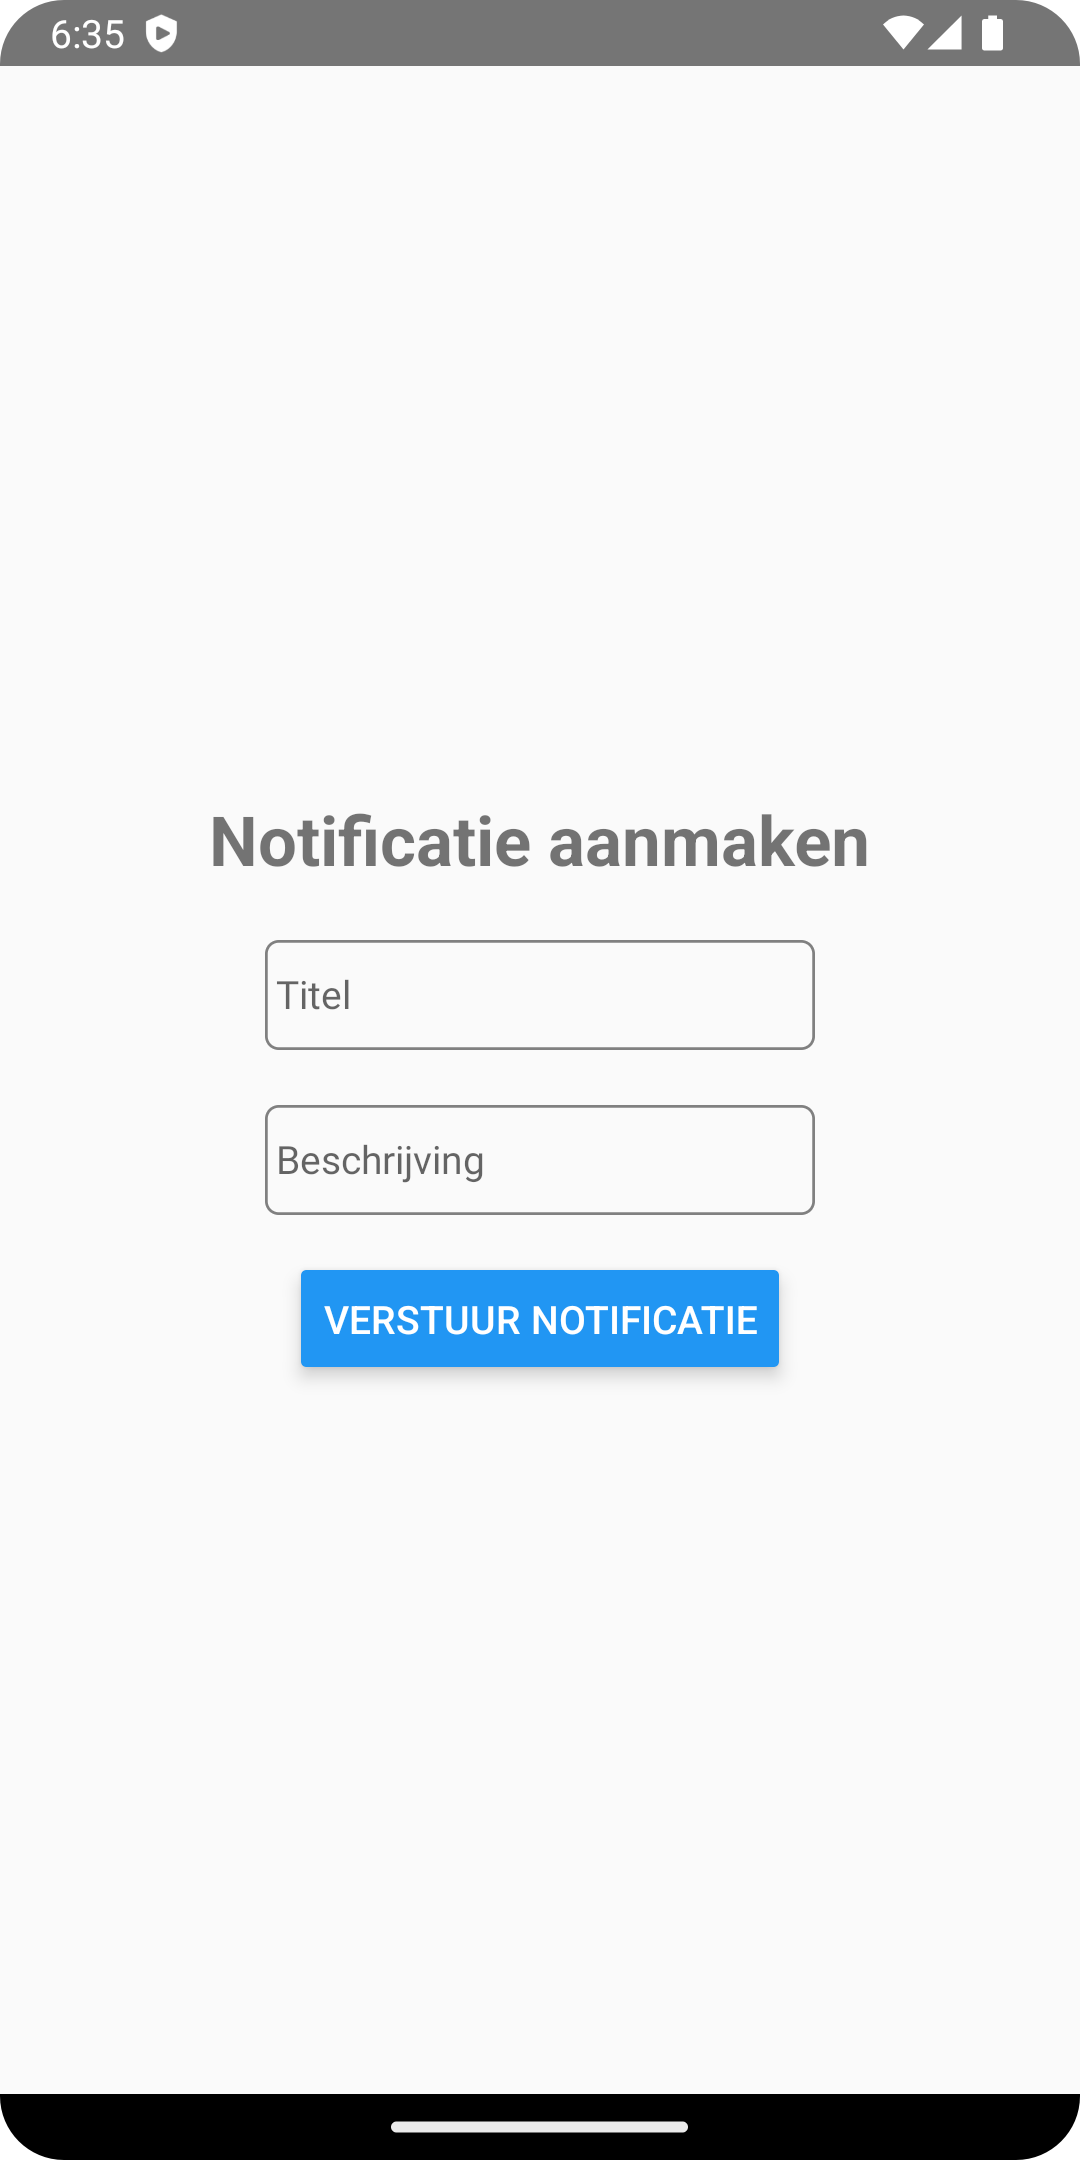
\includegraphics[height=0.5\textheight]{notificaties_layoutcross.png}
  \caption{Layout van applicatie voor notificaties te sturen bij React Native.}
\end{figure}